\documentclass[tikz,border=4pt]{standalone}
\usepackage{pgfplots}
\usepgfplotslibrary{fillbetween}
\pgfplotsset{compat=1.17}
\begin{document}
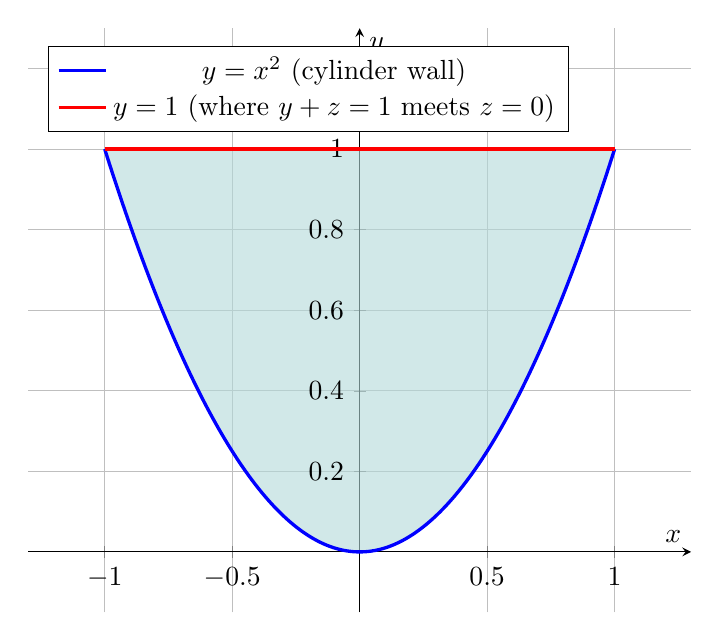
\begin{tikzpicture}
\begin{axis}[
  width=10cm, height=9cm,
  xlabel=$x$, ylabel=$y$,
  xmin=-1.3, xmax=1.3, ymin=-0.15, ymax=1.3,
  axis lines=center,
  samples=150,
  grid=both,
  legend pos=north west
]
\addplot[name path=A, blue, very thick, domain=-1:1]{x^2};
\addplot[name path=B, red, very thick, domain=-1:1]{1};
\addplot[teal!30, opacity=0.6] fill between[of=A and B];
\addlegendentry{$y=x^2$ (cylinder wall)}
\addlegendentry{$y=1$ (where $y+z=1$ meets $z=0$)}
\end{axis}
\end{tikzpicture}
\end{document}
